\chapter{Referencial Teórico}
\label{Referencial_Teorico}


\newcommand{\texCommand}[1]{\texttt{\textbackslash{#1}}}%

\newcommand{\exemplo}[1]{%
\vspace{\baselineskip}%
\noindent\fbox{\begin{minipage}{\textwidth}#1\end{minipage}}%
\\\vspace{\baselineskip}}%

\newcommand{\exemploVerbatim}[1]{%
\vspace{\baselineskip}%
\noindent\fbox{\begin{minipage}{\textwidth}%
#1\end{minipage}}%
\\\vspace{\baselineskip}}%


%%%%%%%%%%%%%%%%%%%%%%%%%%%%%%%%%%%%%%%%%%%%%%%%%%%%%%%%%%%%%%%%%%%%%%%%%%%%%%%%
%%%%%%%%%%%%%%%%%%%%%%%%%%%%%%%%%%%%%%%%%%%%%%%%%%%%%%%%%%%%%%%%%%%%%%%%%%%%%%%%
%%%%%%%%%%%%%%%%%%%%%%%%%%%%%%%%%%%%%%%%%%%%%%%%%%%%%%%%%%%%%%%%%%%%%%%%%%%%%%%%
Este capítulo traz informações sobre metodologias, técnicas e ferramentas computacionais que serão usadas para alcançar os objetivos propostos.
A Seção~\nameref{prototipacao} traz uma breve explicação sobre a metodologia de desenvolvimento de software escolhida.
Na Seção~\nameref{TecDesSof} são explorados os conceitos das tecnologias e ferramentas computacionais empregadas neste trabalho.
A Seção~\nameref{GerProj} descreve o gerenciamento de projetos de análise e desenvolvimento de software abordando algumas diferentes e essenciais etapas como o Levantamento de Requisitos, a Validação e a Implantação.

\section{Prototipação}\label{prototipacao}
\indent

A Prototipação é uma metodologia de desenvolvimento de software cuja principal característica é exibir um protótipo do sistema para o cliente antes de sua implementação~\citep{buchenau2000experience}.
É uma abordagem onde tanto o cliente como o desenvolvedor são beneficiados, uma vez que o cliente pode ter acesso a uma interface prévia do sistema, manifestar sua opinião e discutir funcionalidades desejadas, enquanto o desenvolvedor identifica melhor os requisitos e tem uma maior noção do esforço que será delegado no desenvolvimento~\citep{pressmanengenharia}. 
Usando a prototipação, o processo de software funciona como um ciclo de reuniões entre o cliente e o desenvolvedor e interações com o protótipo ate que haja consenso em uma versão final, conforme exemplificado na Figura~\ref{fig:protPressman}.  

\begin{figure}[htbp]
    \centering
    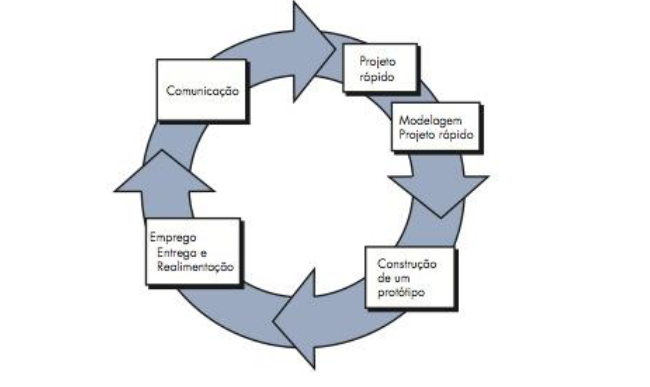
\includegraphics[width=0.75\textwidth]{img/paradigma_prototipacao_pressman.PNG}
    \caption[Paradigma da prototipação]{Paradigma da prototipação. Fonte:~\cite{pressmanengenharia}.}
    \label{fig:protPressman}
\end{figure}

\newpage
\section{Tecnologias de Desenvolvimento de Software}\label{TecDesSof}
\indent

\subsection{\textit{Web}}
\indent

Aplicações \textit{Web} são sistemas cliente/servidor que são acessadas através de um endereço do tipo~\acf{URL} pelo navegador (cliente) que fazem requisições para o servidor~\citep{gonccalves2007}. 
A aplicação pode ser acessada de qualquer dispositivo que tenha internet, independente de \textit{hardware} ou sistema operacionais como Microsoft Windows$^{\circledR}$, Linux diversos, Android, iOS e outros. 

O usuário interage com a aplicação por meio de uma interface processada no navegador e realiza chamadas para o servidor onde está alocada a camada do servidor responsável pelo armazenamento dos dados em conjunto com o banco de dados, e o processamento das regras de negócio~\citep{pereira2018desenvolvimento}.

\subsection{Java}\label{java}
\indent

Java é uma linguagem de programação orientada a objetos, portável, robusta e segura que permite o desenvolvimento de sistemas para a \textit{Web}, \textit{Desktop}, e aparelhos celulares~\citep{mendes2009programaccao}.
Foi criada por James Gosling da Sun Microsystems em 1991, o que chamou atenção na época pois a linguagem podia ser portável para outros sistemas operacionais. Atualmente é utilizada por grandes bancos por ser uma linguagem segura que desfruta de um ecossistema grande e maduro, com forte suporte a ferramentas~\citep{gonccalves2007}. Atualmente o java está na versão 12.0.1
O java possui uma maquina virtual que é conhecida como JVM, ela fornece especificações de \textit{hardware} que permite o java ser uma plataforma independente pois a compilação é feita pela JVM~\citep{mendes2009programaccao}.

\subsection{\textit{Spring Boot}}\label{spring}
\indent

\textit{Spring Boot} é um \textit{framework} criado para agilizar o desenvolvimento de aplicações java pois as configurações necessárias que o desenvolvedor precisa fazer ao iniciar o desenvolvimento de uma aplicação web já vem pre estabelecida, com isso o programador só precisa se preocupar com as regras de negócio~\citep{springboot}.

\subsection{REST}\label{rest}
\indent

\acf{REST} é um modelo de arquitetura para criação de aplicações web que utiliza o protocolo \acf{HTTP} na criação de serviços web com resposta em formato XML ou JSON. 
Uma aplicação é dita RESTful, quando é construída com os princípios básicos do REST~\citep{lecheta2015web}.
O REST tem um conjunto de métodos para a realização das requisições:

\begin{itemize}
    \item \textit{GET} que é utilizado para consulta de dado.
    \item \textit{POST} que é utilizado para inserir dado.
    \item \textit{PUT} que é utilizado para atualização de dado.
    \item \textit{DELETE} que é utilizado para a exclusão de dado.
\end{itemize}

\subsection{Banco de dados}\label{bd}
\indent

Um banco de dados é uma coleção de dados inter-relacionados com a finalidade de fornecer ao usuário o armazenamento dos dados e uma visão abstrata dos dados recuperando-os de maneira eficiente, acessível por sistemas dos mais variados tipos.
O gerenciamento do banco de dados para operações de busca, inserção, atualização e exclusão podem ser realizados por meio de um tipo de software conhecido como \acf{SGBDs}~\citep{silberschatz2016sistema}. 

Existem várias formas de modelar os dados, tais como, o modelo relacional, modelo de entidade/relacionamento, modelo de dados baseado em objeto, modelo de dados semiestruturado entre outros. 
O banco de dados relacional utiliza o modelo relacional que representa os dados e o relacionamento entre eles através de um conjunto de tabelas~\citep{silberschatz2016sistema}.
A linguagem de manipulação dos bancos de dados relacionais é o \acf{SQL}~\citep{silberschatz2016sistema}.

\subsection{MongoDB}\label{mongo}
\indent

Com a utilização em larga escala da \textit{Internet} e com surgimento das redes sociais, o volume de dados vem crescendo rápido.
Com esse crescimento, surgiu a necessidade de manipular e processar grandes quantidades de dados não estruturados, e como solução foi criados os bancos de dados não relacionais ou \acf{NoSQL}. 
O \ac{NoSQL} é um banco não estruturado, flexível com capacidade de escalonamento~\citep{santana2019nosql}. 
Existem vários modelos de dados \ac{NoSQL}, os principais são: Chave-valor, orientado a documentos, orientado a colunas e orientado a grafos~\citep{santana2019nosql}.

MongoDB é um banco de dados não relacional orientada a documento e \textit{open source}, sua representação é simplesmente um conjunto de chave e valor, que permite modificações no documento como adição de novos campos tornando-o flexível e de fácil escalonamento. Os documentos no MongoDB podem ter o tamanho máximo de 16 MB, e utiliza o \acf{JSON} para retornar os resultados das consultas e representar os dados, mas internamente codifica o \ac{JSON} para o \textit{Binary} JSON (BSON). Sua implementação é leve, rápida e eficiente~\citep{mongodb}.
Na Figura~\ref{fig:shell-mongo} é um exemplo de inserção e consulta no \textit{Shell} do MongoDB.

\begin{figure}[H]
    \centering
    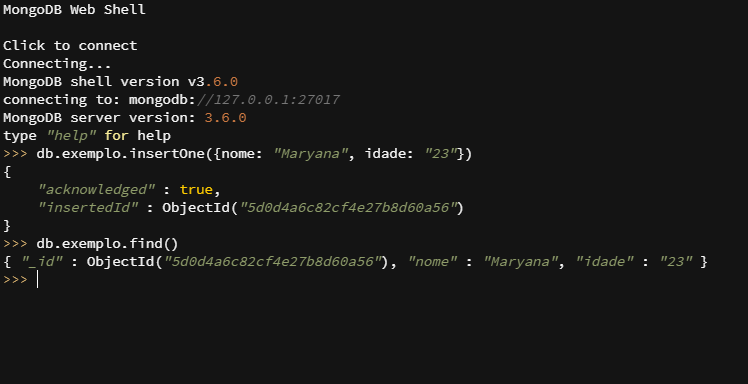
\includegraphics[width=0.95\textwidth]{img/codigo_mongo.PNG}
    \caption[Exemplo no \textit{Shell} do MongoDB]{Exemplo no \textit{Shell} do MongoDB.}
    \label{fig:shell-mongo}
\end{figure}

\subsection{Angular}\label{angular}
\indent

O Angular é um \textit{framework} JavaScript \textit{open source} utilizado na fabricação do \textit{front-end} da aplicação que pode ser tanto web quanto mobile. 
Desenvolvida pela Google, atualmente é um dos \textit{frameworks} mais populares do mercado~\citep{costa2017email}.

\subsection{HTML}\label{html}
\indent

O \acf{HTML} é uma linguagem de marcação que define a estrutura do site que junto com o~\nameref{css} são a base para a construção de páginas web~\citep{w3c}.

\subsection{CSS}\label{css}
\indent

O \acf{CSS} é a linguagem que especifica a apresentação do site como cor, fonte e layout, e é responsável pela a adaptação do site em qualquer tamanho de tela~\citep{w3c}.

\subsection{Bootstrap}\label{bootstrap}
\indent

\textit{Bootstrap} é uma ferramenta \textit{open source} de criação de páginas \textit{Web} responsivas, em conjunto ao~\nameref{html},~\nameref{css} e JavaScript torna fácil o desenvolvimento de sites robustos sem adição de códigos exagerados~\citep{2013bootstrap}.


\section{Gerenciamento de Projetos}\label{GerProj}
\indent

Gerenciamento de projetos é a aplicação de habilidades, ferramentas, conhecimentos e técnicas nas atividades do projeto a fim de cumprir seus requisitos~\citep{pmbok}. 
Ao conjunto de processos e etapas dos projetos de uma organização dá-se o nome de metodologia de gerenciamento, a qual precisa ser adaptada à realidade das organizações~\citep{xavier2005metodologia}.

Nas ultimas décadas, as metodologias ágeis ganharam notoriedade em vários setores do desenvolvimento de software, pois sugerem uma nova perspectiva para o desenvolvimento de projetos.
Metodologias ágeis cortam custos com documentação desnecessária, ressaltando a comunicação e cooperação com o cliente, onde planos detalhados são feitos apenas para a fase atual do projeto, deixando as fases futuras em aberto para adaptações a mudanças, o que pode proporcionar uma qualidade elevada ao sistema~\citep{sato2007uso}.
O termo método ágil está relacionado à eficiência do desenvolvimento e não à velocidade~\citep{prikladnicki2014metodos}.

\textit{Scrum} oferece um \textit{framework} de método ágil com uma estrutura e um conjunto de práticas que mantêm tudo visível permitindo que seja possível saber exatamente o que está acontecendo para fazer ajustes no local para manter o projeto em direção aos objetivos desejados, por meio de reuniões rápidas diárias de acompanhamento do projeto e \textit{sprints} semanais ou mensais~\citep{schwaber2004agile}. 
A visão geral do método scrum é exemplificado na Figura~\ref{fig:scrum}.

No \textit{Scrum} o desenvolvimento do projeto é feita em ciclos, e cada ciclo é chamado de \textit{sprints}, dentro da \textit{sprints} é desenvolvido o que foi planejado para aquele ciclo, quaisquer mudança de requisito ou correção de \textit{bug}, entra nas próximas \textit{sprints}~\citep{pressman2016engenharia}.
Toda e qualquer pessoa que se beneficie do sistema que será desenvolvido é um \textit{Stakeholder}~\citep{pressman2016engenharia}.

\begin{figure}[H]
    \centering
    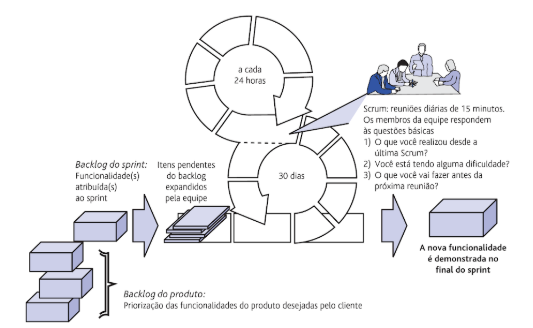
\includegraphics[width=0.95\textwidth]{img/scrum.PNG}
    \caption[Visão geral do método Scrum]{Visão geral do método Scrum. Fonte:~\cite{pressman2016engenharia}.}
    \label{fig:scrum}
\end{figure}

\subsection{Levantamento de requisitos}
\indent

O levantamento de requisitos é um meio apropriado e eficaz de entender aquilo que o cliente deseja e tem como objetivo identificar o problema, propor partes da solução, negociar diferentes abordagens e detalhar um conjunto prévio de requisitos~\citep{pressmanengenharia}. 
O levantamento de requisitos é necessário para uma boa especificação do sistema.
Um bom levantamento de requisitos pode trazer conformidade de tempo e custos do projeto de software. Para tanto, é papel do desenvolvedor insistir e enfatizar que um levantamento adequado, depende entre outros fatores, da efetiva participação do cliente na construção dos requisitos~\citep{de2003engenharia}.

\subsection{Desenvolvimento}
\indent

Depois da prototipação, do levantamento de requisitos e da escolha das tecnologias que serão utilizadas, vem a fase de construção do sistema, onde o desenvolvedor elabora e codifica a aplicação de fato, afim de corresponder ao objetivo do cliente~\citep{pressman2016engenharia}. 
Para se construir um sistema, são escritas uma série de instruções de maneira que o computador e o desenvolvedor entenda e que possa ser executado e transformado em programa~\citep{ascencio2008fundamentos}.

\subsection{Testes e Validação}
\indent

Teste é a atividade que tem como finalidade a execução do sistema de maneira monitorada, com o objetivo de estimar o seu funcionamento baseado no que foi especificado~\citep{rios2006teste}.
Durante o desenvolvimento do sistema falhas no sistema podem acontecer, ou uma funcionalidade pode ser mal construída sem que o programador perceba, com a realização de testes é possível detectar falhas ou comportamentos indesejáveis. 
É realizada a verificação do correto funcionamento das funcionalidades e a validação dos requisitos especificado pelo cliente~\citep{costa2006estrategia}.


\subsection{Implantação}
\indent

A implantação do sistema tem como característica principal a disponibilização do software em perfeito funcionamento. 
Esta é a ultima fase do projeto, que é conhecida também como "prova de fogo", pois é nessa etapa que o cliente recebe o resultado final de todo o projeto. O objetivo é realizar uma implantação com sucesso, e caso necessário elaborar manual de utilização do sistema, e realizar treinamento com o usuário final para que se obtenha a total satisfação do cliente~\citep{rezende2006engenharia}.